%%==================================================
%% chapter5.tex for BIT Master Thesis
%% version: 0.1
%% last update: Nov 8th, 2017
%%==================================================
\chapter{半参数自适应运动控制}\label{chap:5}
反馈控制是为解决实际问题而研究设计的。前面几章针对一种典型先验信息和数学描述的模型设计了半参数自适应估计与控制器,并用数值仿真验证了控制器性能。本章将考虑半参数自适应控制引入到运动控制场景,解决多关节机械臂中伺服电机的控制问题。
\section{问题描述}
\subsection{机器人控制问题}
一般来说,机器人是一个复杂的多输入、多输出非线性系统,具有时变、强耦合和非线性的动力学特征。机器人运动学和动力学的非线性和耦合性使得机器人控制系统的设计十分复杂,一般来说,将如图\ref{fig.robot}所示机器人(机械臂)的运动控制分成两个阶段分别优化,即任务空间的轨迹(路径)规划和关节空间的跟踪控制\upcite{ShinMckay1986}。前者轨迹(路径)规划部分性能的提高涉及到运动学甚至障碍物等约束等多种综合因素的考量,轨迹规划器最终会给后者跟踪控制以关节空间形式提供一段期望的运行轨迹。本章主要考虑关节空间的跟踪控制问题。

\begin{figure}[!htb]
	\centering
	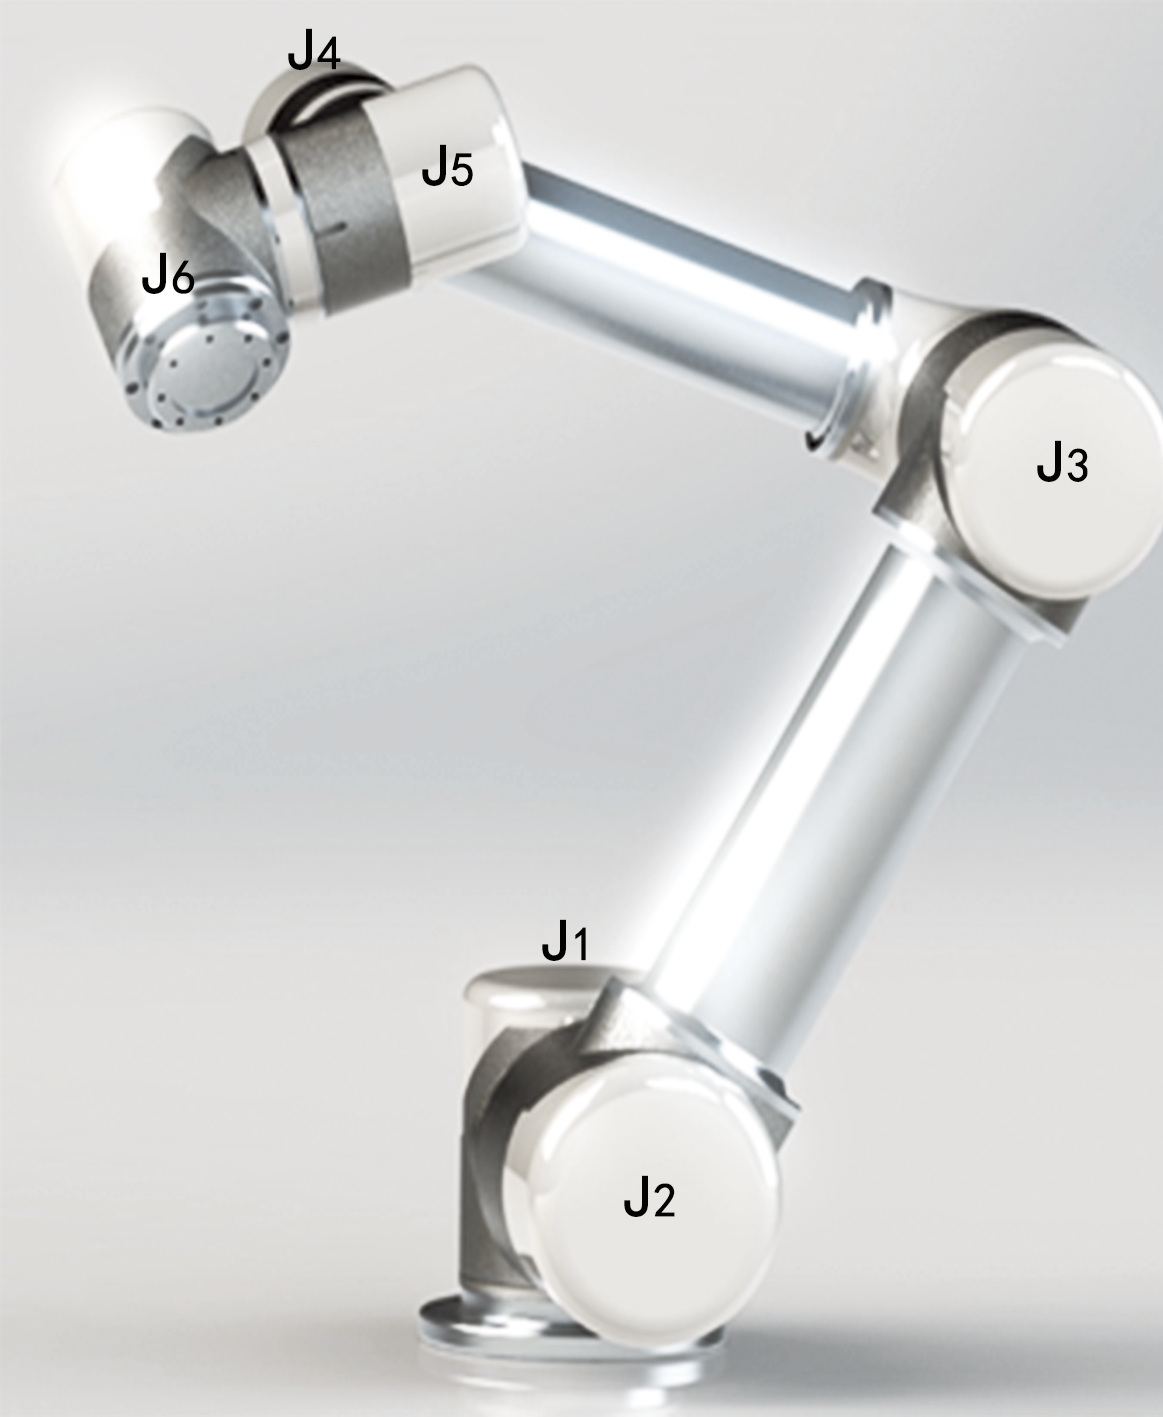
\includegraphics[width=0.35\textwidth ]{ch5-ur-robot.png}\\	 % e.g.,[scale=0.75], [width=0.75\textwidth ]
	\caption{一种UR构型的协作机器人}
	\label{fig.robot}
\end{figure}

工程应用中由于建模和测量的不准确,加上负载的变化以及外部扰动的影响,实际上难以获得机器人精确完整的运动学模型。因此机器人的控制系统中存在的不确定性因素主要可以分为两类,第一类是参数不确定性,如负载质量、连杆长度、连杆质心等物理量未知或部分已知;第二类是非参数不确定性,如高频未建模动态,包括驱动器动力学、结构共振模式,以及低频难以建模动态,如动态/静态摩擦力、关节柔性等。

\subsection{伺服电机控制问题}

\section{仿真实例}

\section{本章总结}
本章主要介绍了